\documentclass[9pt,a4paper]{extarticle}
\usepackage{parskip}

\usepackage[utf8]{inputenc}
\usepackage[T1]{fontenc}
% Nota: em instalações mais antigas do TeX Live, troque a linha abaixo por \usepackage[brazil]{babel}
\usepackage[brazilian,provide=*]{babel}
\usepackage{amsmath, amssymb, amsthm}
\usepackage{geometry}
\usepackage{listings}
\usepackage{xcolor}
\usepackage{hyperref}
\usepackage{booktabs}
\usepackage{array}
\usepackage{tabularx}
\usepackage{enumitem}
\usepackage[expansion=false]{microtype}
\usepackage{csquotes}
\usepackage{natbib}
\usepackage{tikz}
\usetikzlibrary{positioning,arrows.meta}

\definecolor{important}{RGB}{255, 100, 100}
\definecolor{notice}{RGB}{0, 102, 204}
\definecolor{maccent}{RGB}{230, 120, 30}

\newcommand{\impt}[1]{\textcolor{important}{\textbf{#1}}}
\newcommand{\ntc}[1]{\textcolor{notice}{#1}}

\setlist{nosep}
\geometry{margin=2cm}

\newtheorem{theorem}{Teorema}[section]
\newtheorem{lemma}[theorem]{Lema}
\newtheorem{corollary}[theorem]{Corolário}
\theoremstyle{definition}
\newtheorem{definition}{Definição}[section]
\newtheorem{example}{Exemplo}[section]
\newtheorem{remark}{Observação}[section]

\title{NP-Completude: uma reorganização didática\footnote{Material baseado em \citep{clrs2009}, com referência aos trabalhos originais de \citet{cook1971}, \citet{karp1972} e \citet{garey1979}. A ordem de apresentação aqui difere deliberadamente da seção 34 de \citet{clrs2009}: o formalismo de codificações/problemas abstratos é reduzido ao mínimo necessário, a intuição de reduções é construída antes da definição formal, e a demonstração de Cook-Levin é tratada como resultado de \enquote{caixa-preta}, com foco no uso prático das reduções e no que fazer diante de um problema NP-completo.}}
\author{PCC104 -- Projeto e Análise de Algoritmos}
\date{\today}

\begin{document}
\maketitle
\tableofcontents

\section{Motivação: por que precisamos disso}\label{sec:motivacao}

Até aqui, vimos uma sequência de problemas que admitem algoritmos eficientes: ordenação (\(O(n\log n)\)), caminho mínimo (Dijkstra, \(O(E + V\log V)\)), fluxo máximo, árvore geradora mínima. Em todos esses casos, o tempo de execução cresce como um polinômio no tamanho da entrada, e essa é precisamente a noção que usamos para dizer que um problema é \impt{tratável na prática}.

Mas existe uma classe de problemas, estruturalmente muito parecidos com os anteriores, para os quais \emph{ninguém jamais encontrou} um algoritmo polinomial -- apesar de décadas de tentativas por parte de gente muito competente. Compare:

\begin{center}
\begin{tabular}{@{}p{6.2cm}p{6.2cm}@{}}
\toprule
\textbf{Fácil (em P)} & \textbf{Aparentemente difícil} \\
\midrule
Existe um \emph{caminho} de \(s\) a \(t\) com no máximo \(k\) arestas? (BFS, \(O(V+E)\)) & Existe um \emph{caminho simples} (sem repetir vértices) de \(s\) a \(t\) que passe por \emph{todos} os vértices? (\textsc{Ham-Path}) \\[2pt]
Existe um circuito de Euler (percorre toda \emph{aresta} exatamente uma vez)? (\(O(V+E)\)) & Existe um ciclo hamiltoniano (visita todo \emph{vértice} exatamente uma vez)? (\textsc{Ham-Cycle}) \\[2pt]
\textsc{2-Sat}: fórmula booleana em FNC\footnotemark{} com 2 literais por cláusula é satisfazível? (\(O(n+m)\), via componentes fortemente conexas) & \textsc{3-Sat}: mesma pergunta, com 3 literais por cláusula \\
\bottomrule
\end{tabular}
\end{center}
\footnotetext{FNC, literal e cláusula serão definidos formalmente na Definição~\ref{def:fnc}; por ora, basta a ideia: uma fórmula que é um \enquote{E} de cláusulas, cada cláusula um \enquote{OU} de variáveis possivelmente negadas.}

A diferença de enunciado é mínima. A diferença de dificuldade prática é gigantesca. Isso não é acidente -- é o objeto de estudo desta aula.

\paragraph{Por que isso importa na prática?} Problemas como escalonamento de tarefas, roteamento de veículos, alocação de recursos, design de circuitos e bioinformática recaem, quase todos, nessa categoria difícil. Um profissional que não reconhece um problema NP-completo corre o risco de gastar meses tentando achar um algoritmo polinomial que (com altíssima probabilidade) não existe, em vez de partir direto para heurísticas, aproximações ou formulações exatas com solvers especializados.

\begin{table}[h]
\centering
\begin{tabular}{@{}rrr@{}}
\toprule
\(n\) & \(n^3\) (polinomial) & \(2^n\) (exponencial) \\
\midrule
10 & 1.000 & 1.024 \\
20 & 8.000 & 1.048.576 \\
30 & 27.000 & \(\approx 10^9\) \\
50 & 125.000 & \(\approx 10^{15}\) \\
60 & 216.000 & \(\approx 10^{18}\) (idade do universo em segundos: \(\approx 4\times10^{17}\)) \\
\bottomrule
\end{tabular}
\caption{Crescimento polinomial vs. exponencial. Para \(n=60\), um algoritmo exponencial já é impraticável mesmo em supercomputadores.}
\end{table}

\impt{O objetivo desta aula} não é provar que \(P \neq NP\) -- isso é um problema em aberto, um dos Problemas do Milênio do Clay Mathematics Institute. O objetivo é: (i) formalizar a diferença entre \enquote{fácil de resolver} e \enquote{fácil de verificar}; (ii) aprender a técnica de \emph{reduções} para provar que um problema é \enquote{tão difícil quanto} outro; (iii) saber reconhecer um problema NP-completo quando você encontrar um; (iv) saber o que fazer depois de reconhecê-lo.

\section{Problemas de decisão e a classe P}\label{sec:classe-p}

Para comparar problemas entre si de forma rigorosa, é conveniente reduzir todo problema a uma pergunta de \impt{sim/não}.

\paragraph{Notação.} Denotamos por \(\{0,1\}^*\) o conjunto de todas as \ntc{cadeias binárias finitas} (incluindo a cadeia vazia): \(\{0,1\}^* = \{\varepsilon, 0, 1, 00, 01, 10, 11, 000, \dots\}\). Para uma cadeia \(x \in \{0,1\}^*\), \(|x|\) denota seu comprimento em bits.

\begin{definition}[Problema de decisão]
Um problema de decisão é uma função \(f: \{0,1\}^* \to \{0,1\}\). Formalmente, identificamos o problema com a \impt{linguagem} \(L = \{x \in \{0,1\}^* : f(x) = 1\}\) -- o conjunto das instâncias codificadas cuja resposta é \enquote{sim}. Dizemos que um algoritmo \impt{decide} \(L\) se, para toda entrada \(x\), ele responde corretamente se \(x \in L\) ou \(x \notin L\).
\end{definition}

\begin{example}\label{ex:decisao-otimizacao}
\textsc{Path}: dado um grafo \(G\), vértices \(u,v\) e inteiro \(k\), existe caminho de \(u\) a \(v\) com no máximo \(k\) arestas? A versão de otimização (\enquote{qual o comprimento do caminho mínimo?}) é equivalente em dificuldade, no seguinte sentido: quem resolve a otimização resolve a decisão de graça (compare o mínimo com \(k\)); e quem resolve a decisão resolve a otimização com busca binária sobre \(k\) -- um número apenas polinomial de chamadas. Por isso, restringir a teoria a problemas de decisão \emph{não perde generalidade} para nossos fins.
\end{example}

\ntc{Toda entrada -- grafo, fórmula booleana, conjunto de números -- é assumida codificada como uma cadeia de bits por um esquema de codificação razoável (sem \emph{blow-up} exponencial: números em binário, não em unário). Não vamos nos aprofundar nesse ponto -- ele é relevante apenas para evitar patologias como o algoritmo pseudo-polinomial de \textsc{Subset-Sum}, que reencontraremos na Seção~\ref{sec:receita}.}

\begin{definition}[Classe P]
\(P\) é o conjunto das linguagens \(L\) para as quais existe um algoritmo que decide \(L\) em tempo \(O(n^k)\) para alguma constante \(k\), onde \(n = |x|\) é o tamanho da entrada.
\end{definition}

\(P\) é o nosso modelo formal de \enquote{tratável}. Tudo que vimos no curso até agora está em \(P\).

\section{A classe NP: fácil de \emph{verificar}}\label{sec:classe-np}

Considere \textsc{Ham-Cycle}: dado um grafo \(G\), existe um \impt{ciclo hamiltoniano} -- um ciclo simples que visita cada vértice de \(G\) exatamente uma vez? Ninguém conhece algoritmo polinomial para resolver isso. Mas note uma assimetria interessante: \emph{se alguém te der um ciclo candidato}, verificar se ele é de fato hamiltoniano é trivialíssimo -- percorra a sequência de vértices, confira que cada aresta consecutiva existe no grafo e que cada vértice aparece exatamente uma vez. Isso é \(O(V+E)\).

Essa assimetria -- difícil de \emph{resolver}, fácil de \emph{verificar dada uma resposta pronta} -- é o conceito central desta seção.

\begin{definition}[Verificador]\label{def:verificador}
Um algoritmo \(A(x,y)\) de duas entradas é um \impt{verificador} para a linguagem \(L\) se
\[
L = \{x \in \{0,1\}^* : \exists\, y \in \{0,1\}^* \text{ com } |y| = O(|x|^c),\ A(x,y) \text{ aceita}\},
\]
para alguma constante \(c\). Chamamos \(y\) de \impt{certificado} (ou testemunha). \(A\) é um \impt{verificador de tempo polinomial} se roda em tempo polinomial em \(|x|\). Note que exigimos o certificado curto (\(|y|\) polinomial em \(|x|\)); sem essa exigência, o verificador nem conseguiria ler \(y\) inteiro em tempo polinomial em \(|x|\).
\end{definition}

\begin{definition}[Classe NP]
\(NP\) é o conjunto das linguagens que possuem um verificador de tempo polinomial.
\end{definition}

Em palavras: \(L \in NP\) se toda instância \enquote{sim} de \(L\) possui uma \emph{prova curta e rapidamente checável} de que a resposta é sim. Nada é dito sobre instâncias \enquote{não} -- para elas, pode não existir prova curta nenhuma.

\begin{example}
Para \textsc{Ham-Cycle}, o certificado \(y\) é a própria sequência de vértices do ciclo proposto. Para \textsc{Clique} (\(G\) tem um subconjunto de \(k\) vértices mutuamente adjacentes?), o certificado é o próprio subconjunto de vértices -- o verificador testa os \(\binom{k}{2}\) pares. Para \textsc{Sat} (uma fórmula booleana tem atribuição de valores-verdade que a torna verdadeira?), o certificado é a atribuição -- o verificador avalia a fórmula.
\end{example}

\begin{remark}
\(NP\) \emph{não} significa \enquote{não-polinomial} -- é um erro de leitura comum. \(NP\) = \emph{Nondeterministic Polynomial time}: o nome vem de uma definição equivalente via máquinas de Turing não-determinísticas, que \enquote{adivinham} o certificado. Preferimos aqui a definição via verificador, mais intuitiva.
\end{remark}

\begin{theorem}
\(P \subseteq NP\).
\end{theorem}
\begin{proof}[Ideia]
Se \(L \in P\), construa um verificador que ignora \(y\) e decide \(x\) diretamente com o algoritmo polinomial de \(L\). Certificado vazio, verificação trivialmente correta.
\end{proof}

\ntc{A grande pergunta em aberto: \(P = NP\)? Isto é, será que todo problema fácil de verificar é também fácil de resolver? A crença quase unânime da comunidade é que \(P \neq NP\), mas ninguém sabe provar. O restante desta aula constrói a maquinaria para identificar os problemas \emph{mais difíceis} de \(NP\) -- se qualquer um deles cair em \(P\), então \(P = NP\).}

\section{Reduções em tempo polinomial}\label{sec:reducoes}

Antes de qualquer definição formal, um exemplo concreto. Considere dois problemas:

\begin{itemize}
\item \textsc{Clique}\((G,k)\): \(G\) tem um subconjunto de \(k\) vértices todos mutuamente adjacentes?
\item \textsc{Independent-Set}\((G,k)\): \(G\) tem um subconjunto de \(k\) vértices em que \emph{nenhum} par é adjacente?
\end{itemize}

Seja \(\bar G\) o \impt{grafo complementar} de \(G\): mesmo conjunto de vértices, e \(u,v\) são adjacentes em \(\bar G\) se, e somente se, \emph{não} são adjacentes em \(G\). É imediato que:
\[
G \text{ tem clique de tamanho } k \iff \bar G \text{ tem conjunto independente de tamanho } k,
\]
pois um conjunto de vértices é totalmente conectado em \(G\) exatamente quando é totalmente desconectado em \(\bar G\).

Isso nos dá uma transformação: dado \((G,k)\), calcule \(\bar G\) (tempo \(O(V^2)\), certamente polinomial) e pergunte sobre \((\bar G, k)\). \impt{A resposta é a mesma para os dois problemas.} Chamamos isso de \emph{redução}.

\begin{definition}[Redução em tempo polinomial]\label{def:reducao}
Dizemos que \(L_1 \leq_p L_2\) (\(L_1\) \impt{reduz em tempo polinomial} a \(L_2\)) se existe uma função \(f: \{0,1\}^* \to \{0,1\}^*\), computável em tempo polinomial, tal que
\[
x \in L_1 \iff f(x) \in L_2, \quad \text{para todo } x \in \{0,1\}^*.
\]
A leitura intuitiva do símbolo: \(L_1 \leq_p L_2\) significa \enquote{\ntc{\(L_1\) não é mais difícil que \(L_2\)}} -- quem sabe resolver \(L_2\) automaticamente sabe resolver \(L_1\).
\end{definition}

\begin{theorem}\label{thm:reducao-transfere}
Se \(L_1 \leq_p L_2\) e \(L_2 \in P\), então \(L_1 \in P\).
\end{theorem}
\begin{proof}
Para decidir \(x \in L_1\): calcule \(f(x)\) (tempo polinomial) e decida se \(f(x) \in L_2\) (tempo polinomial, pois \(L_2 \in P\)). Um detalhe que merece atenção: como \(f\) roda em tempo polinomial em \(|x|\), sua saída satisfaz \(|f(x)| = O(|x|^c)\) -- um algoritmo não consegue escrever mais símbolos do que o tempo de que dispõe. Assim, o custo do segundo passo é polinomial em \(|f(x)|\), que é polinomial em \(|x|\); e a composição de polinômios é um polinômio.
\end{proof}

\impt{Este é o único fato que você precisa para entender por que reduções importam.} Leia o Teorema~\ref{thm:reducao-transfere} na contrapositiva: \ntc{se \(L_1 \notin P\), então \(L_2 \notin P\)}. Ou seja: \emph{reduzir \(L_1\) a \(L_2\) transfere a dificuldade de \(L_1\) para \(L_2\)}.

\begin{remark}[O erro mais comum de estudante]\label{rem:direcao}
A direção da redução importa, e é contraintuitiva na primeira vez. Para provar que \(L_2\) é \emph{difícil}, você reduz um problema \emph{já conhecido como difícil} \emph{para} \(L_2\) (ou seja, mostra \(L_1 \leq_p L_2\) com \(L_1\) sabidamente difícil). Você \textbf{não} reduz \(L_2\) para outra coisa -- isso só mostraria que \(L_2\) é \emph{fácil demais}, não que é difícil. A pergunta que a redução responde é: \enquote{se eu soubesse resolver \(L_2\) rapidamente, eu resolveria \(L_1\) rapidamente também?}. Se sim, \(L_2\) é pelo menos tão difícil quanto \(L_1\).
\end{remark}

\begin{lemma}[Transitividade]\label{lem:transitividade}
Se \(L_1 \leq_p L_2\) e \(L_2 \leq_p L_3\), então \(L_1 \leq_p L_3\).
\end{lemma}
\begin{proof}[Ideia]
Componha as duas funções de redução; pelo mesmo argumento do Teorema~\ref{thm:reducao-transfere}, a composição ainda é computável em tempo polinomial.
\end{proof}

Essa transitividade é o que vai nos permitir construir \emph{cadeias} de reduções na Seção~\ref{sec:receita}, sem provar cada problema \enquote{do zero}.

\section{NP-completude: definição}\label{sec:npc}

Agora podemos formalizar a noção de \enquote{problema mais difícil de \(NP\)}.

\begin{definition}[NP-completo e NP-difícil]\label{def:npc}
Uma linguagem \(L\) é \impt{NP-difícil} (\emph{NP-hard}) se \(L' \leq_p L\) para \emph{toda} linguagem \(L' \in NP\). Uma linguagem \(L\) é \impt{NP-completa} se, além de NP-difícil, também vale \(L \in NP\).

Note: NP-difícil \emph{não} exige pertencer a \(NP\) -- existem problemas NP-difíceis que (acredita-se) estão fora de \(NP\), como a versão de otimização do TSP ou o problema da parada. Os NP-completos são exatamente os NP-difíceis que ainda vivem dentro de \(NP\).
\end{definition}

\begin{theorem}\label{thm:npc-implica-pnp}
Se algum problema NP-completo \(L\) está em \(P\), então \(P = NP\).
\end{theorem}
\begin{proof}[Ideia]
Por definição de NP-completude, todo \(L' \in NP\) satisfaz \(L' \leq_p L\). Se \(L \in P\), pelo Teorema~\ref{thm:reducao-transfere}, \(L' \in P\) para todo \(L' \in NP\). Logo \(NP \subseteq P\); como já sabemos \(P \subseteq NP\), segue \(P = NP\).
\end{proof}

Este teorema é a razão de todo o interesse prático da NP-completude: \impt{os problemas NP-completos são, coletivamente, os \enquote{elos mais fracos} de \(NP\)} -- resolver qualquer um em tempo polinomial resolveria todos. Como décadas de tentativas falharam para \emph{milhares} de problemas NP-completos catalogados \citep{garey1979}, a crença de que \(P \neq NP\) se fortalece a cada tentativa fracassada.

\begin{corollary}\label{cor:mostrar-npc}
Para mostrar que \(L\) é NP-completo, basta:
\begin{enumerate}
\item mostrar \(L \in NP\) (exibir um verificador polinomial); \textbf{e}
\item exibir \emph{um único} problema \(L'\) já conhecido como NP-completo e mostrar \(L' \leq_p L\).
\end{enumerate}
\end{corollary}
\begin{proof}[Por que basta um único \(L'\)?]
Como \(L'\) é NP-completo, todo \(L'' \in NP\) satisfaz \(L'' \leq_p L'\). Se também \(L' \leq_p L\), a transitividade (Lema~\ref{lem:transitividade}) dá \(L'' \leq_p L\) para todo \(L'' \in NP\). Ou seja, um único \enquote{elo} basta para herdar as reduções de \emph{todos} os problemas de \(NP\) simultaneamente.
\end{proof}

O Corolário~\ref{cor:mostrar-npc} é a técnica que vamos aplicar repetidamente na Seção~\ref{sec:receita}. Mas ele tem um problema de \enquote{ovo e galinha}: precisamos de \emph{pelo menos um} problema NP-completo estabelecido \enquote{do zero} -- provando a condição (2) da Definição~\ref{def:npc} diretamente, contra todos os infinitos problemas de \(NP\) de uma vez -- para começar a cadeia. Esse é o papel do teorema da próxima seção.

\section{O Teorema de Cook-Levin (como caixa-preta)}\label{sec:cook-levin}

\begin{theorem}[Cook--Levin, \citealp{cook1971}]\label{thm:cook-levin}
\textsc{Circuit-Sat} é NP-completo, onde \textsc{Circuit-Sat}\((C)\) pergunta: dado um circuito booleano \(C\) com portas \emph{AND}, \emph{OR} e \emph{NOT}, existe uma atribuição das entradas que faz a saída de \(C\) ser 1?
\end{theorem}

\ntc{Não vamos demonstrar este teorema linha a linha -- a prova completa está em \citet[Seção 34.3--34.4]{clrs2009} para quem quiser se aprofundar. O que importa \emph{para usar} o resultado é a ideia central:}

\paragraph{Ideia da prova.} \(\textsc{Circuit-Sat} \in NP\) é fácil: o certificado é a própria atribuição de entradas, e simular o circuito com essa atribuição é polinomial. A parte difícil é a segunda condição: mostrar que \emph{todo} \(L \in NP\) reduz a \textsc{Circuit-Sat}. A observação-chave é que um verificador polinomial \(A(x,y)\) é, ele mesmo, um programa que roda em tempo polinomial -- e todo programa que roda em tempo \(T\) pode ser simulado por um circuito booleano de tamanho polinomial em \(T\), essencialmente \enquote{desenrolando} a sequência de configurações da máquina passo a passo em portas lógicas. O circuito resultante recebe \(x\) fixado (\enquote{cravado} nos fios de entrada correspondentes) e \(y\) como entradas livres; ele é satisfazível \emph{exatamente quando} existe \(y\) que faz \(A(x,y)\) aceitar -- ou seja, exatamente quando \(x \in L\). Essa construção do circuito a partir do verificador é, ela mesma, computável em tempo polinomial, como a Definição~\ref{def:reducao} exige.

\begin{corollary}
\textsc{Circuit-Sat} é o \enquote{problema-semente}: a partir dele, o Corolário~\ref{cor:mostrar-npc} nos permite provar a NP-completude de qualquer outro problema exibindo apenas uma redução, sem repetir o argumento de simulação de máquinas por circuitos.
\end{corollary}

\section{A receita prática e a cadeia de reduções}\label{sec:receita}

Toda prova de NP-completude por redução segue o mesmo roteiro, e vale a pena nomeá-lo antes dos exemplos. Para provar que \(L\) é NP-completo:

\begin{enumerate}
\item \impt{Mostre \(L \in NP\)} (geralmente trivial: exiba o certificado e o verificador).
\item \impt{Escolha um \(L'\) NP-completo já conhecido}, estruturalmente parecido com \(L\), e monte a redução \emph{na direção certa}: \(L' \leq_p L\) (releia a Observação~\ref{rem:direcao} se necessário).
\item \impt{Construa \(f\)}: uma transformação polinomial de instâncias de \(L'\) para instâncias de \(L\), tipicamente por meio de \impt{gadgets} -- pedaços da instância de \(L\) que \enquote{imitam} peças da instância de \(L'\) (uma cláusula vira um triplo de vértices; uma variável vira um par de números; etc.).
\item \impt{Prove a correção nas duas direções}: (a) se \(x\) é instância \enquote{sim} de \(L'\), então \(f(x)\) é instância \enquote{sim} de \(L\); \textbf{e} (b) se \(f(x)\) é instância \enquote{sim} de \(L\), então \(x\) é instância \enquote{sim} de \(L'\). \ntc{Estudantes costumam provar só a direção (a) e esquecer a (b) -- ambas são obrigatórias, pois a Definição~\ref{def:reducao} exige um \enquote{se, e somente se}.}
\end{enumerate}

Antes das reduções, definimos formalmente os problemas envolvidos.

\begin{definition}[FNC, literal, cláusula]\label{def:fnc}
Um \impt{literal} é uma variável booleana \(x\) ou sua negação \(\bar x\) (também escrita \(\neg x\)). Uma \impt{cláusula} é uma disjunção (OU) de literais, ex.\ \((x_1 \vee \bar x_2 \vee x_3)\). Uma fórmula está em \impt{forma normal conjuntiva (FNC)} se é uma conjunção (E) de cláusulas: \(\phi = C_1 \wedge C_2 \wedge \dots \wedge C_k\). A fórmula é \impt{satisfazível} se existe uma atribuição de valores-verdade às variáveis que a torna verdadeira -- ou seja, que torna verdadeiro ao menos um literal em \emph{cada} cláusula.
\end{definition}

\begin{definition}[Os problemas da cadeia]\label{def:problemas}
\begin{itemize}
\item \textsc{Sat}\((\phi)\): a fórmula booleana \(\phi\) (qualquer) é satisfazível?
\item \textsc{3-Cnf-Sat}\((\phi)\): a fórmula \(\phi\), em FNC com \emph{exatamente 3 literais por cláusula}, é satisfazível?
\item \textsc{Clique}\((G,k)\): \(G\) tem clique de tamanho \(k\)?
\item \textsc{Vertex-Cover}\((G,k)\): existe \(V' \subseteq V\), \(|V'| \leq k\), tal que toda aresta de \(G\) tem ao menos uma ponta em \(V'\)? (\(V'\) é uma \emph{cobertura de vértices}.)
\item \textsc{Ham-Cycle}\((G)\): \(G\) tem ciclo hamiltoniano?
\item \textsc{Tsp}\((G,w,k)\): dado grafo completo \(G\) com pesos \(w\) nas arestas e inteiro \(k\), existe uma \emph{turnê} (ciclo hamiltoniano) de custo total \(\leq k\)? (Versão de decisão do caixeiro-viajante.)
\item \textsc{Subset-Sum}\((S,t)\): dado um conjunto finito \(S\) de inteiros positivos e um alvo \(t\), existe subconjunto \(S' \subseteq S\) com \(\sum_{s \in S'} s = t\)?
\end{itemize}
\end{definition}

A cadeia clássica, montada por \citet{karp1972} e adaptada de \citet[Seção 34.5]{clrs2009}:

\begin{center}
\begin{tikzpicture}[every node/.style={font=\scriptsize}, >={Stealth[length=2mm]}]
\node (csat) at (0,0) {\textsc{Circuit-Sat}};
\node (sat) at (2.5,0) {\textsc{Sat}};
\node (3sat) at (4.6,0) {\textsc{3-Cnf-Sat}};
\node (clique) at (7.3,0.65) {\textsc{Clique}};
\node (vc) at (9.8,0.65) {\textsc{Vertex-Cover}};
\node (ham) at (12.5,0.65) {\textsc{Ham-Cycle}};
\node (tsp) at (14.4,0.65) {\textsc{Tsp}};
\node (ssum) at (7.3,-0.85) {\textsc{Subset-Sum}};
\draw[->] (csat) -- (sat);
\draw[->] (sat) -- (3sat);
\draw[->] (3sat) -- (clique);
\draw[->] (clique) -- (vc);
\draw[->] (vc) -- (ham);
\draw[->] (ham) -- (tsp);
\draw[->] (3sat) -- (ssum);
\end{tikzpicture}
\end{center}

Cada seta \(L' \to L\) é uma redução \(L' \leq_p L\); pela transitividade e pelo Corolário~\ref{cor:mostrar-npc}, todos os nós da cadeia são NP-completos (cada um está em \(NP\) -- verifique mentalmente qual é o certificado de cada um). Vamos detalhar as duas primeiras reduções da cadeia \emph{de grafos} por completo -- são as mais instrutivas sobre a técnica de gadgets -- e esboçar as demais.

\subsection{\textsc{3-Cnf-Sat} \(\leq_p\) \textsc{Clique} (completa)}\label{sec:3sat-clique}

Seja \(\phi = C_1 \wedge C_2 \wedge \dots \wedge C_k\) uma fórmula em FNC com exatamente 3 literais por cláusula.

\paragraph{Construção do gadget.} Para cada cláusula \(C_i = (\ell_1^i \vee \ell_2^i \vee \ell_3^i)\), crie um \impt{triplo de vértices} \(v_1^i, v_2^i, v_3^i\), um para cada literal. Ligue \(v_p^i\) a \(v_q^j\) por uma aresta se, e somente se: (a) estão em triplos diferentes (\(i \neq j\)); \textbf{e} (b) os literais correspondentes não são complementares (não é o caso de um ser \(x\) e o outro \(\bar x\), para a mesma variável \(x\)). A instância de \textsc{Clique} produzida é \((G, k)\), com \(k\) = número de cláusulas de \(\phi\).

\begin{example}[Instância concreta]\label{ex:3sat-clique}
Considere \(\phi = (x_1 \vee x_2 \vee \bar x_3) \wedge (\bar x_1 \vee \bar x_2 \vee x_3)\), com \(k=2\) cláusulas. O grafo construído tem 6 vértices e as arestas mostradas abaixo (note as \emph{não}-arestas: pares dentro do mesmo triplo e pares complementares \(x_1\)--\(\bar x_1\), \(x_2\)--\(\bar x_2\), \(\bar x_3\)--\(x_3\)):

\begin{center}
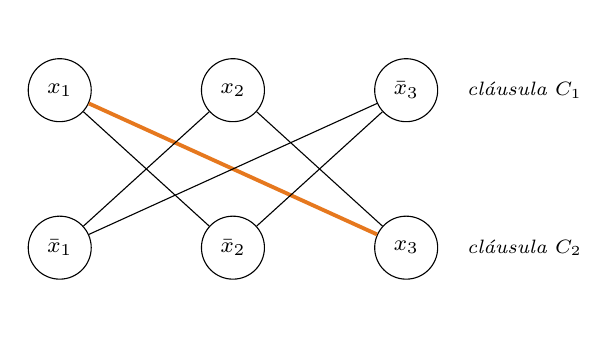
\begin{tikzpicture}[every node/.style={circle, draw, font=\footnotesize, inner sep=1.5pt, minimum size=8mm}]
% Triplo da cláusula 1 (em cima)
\node (a1) at (0,2)   {\(x_1\)};
\node (a2) at (2.2,2) {\(x_2\)};
\node (a3) at (4.4,2) {\(\bar x_3\)};
% Triplo da cláusula 2 (embaixo)
\node (b1) at (0,0)   {\(\bar x_1\)};
\node (b2) at (2.2,0) {\(\bar x_2\)};
\node (b3) at (4.4,0) {\(x_3\)};
% Arestas (entre triplos, literais não complementares)
\draw[line width=1.4pt, color=maccent] (a1) -- (b3); % clique destacada
\draw (a1) -- (b2);
\draw (a2) -- (b1);
\draw (a2) -- (b3);
\draw (a3) -- (b1);
\draw (a3) -- (b2);
% Rótulos dos triplos
\node[draw=none, font=\scriptsize\itshape] at (5.9,2) {cláusula \(C_1\)};
\node[draw=none, font=\scriptsize\itshape] at (5.9,0) {cláusula \(C_2\)};
\end{tikzpicture}
\end{center}

Uma clique de tamanho \(k=2\) é qualquer aresta; a destacada em laranja, \(\{x_1, x_3\}\), corresponde à atribuição \(x_1 = \mathrm{V}\), \(x_3 = \mathrm{V}\) (e \(x_2\) com valor arbitrário), que de fato satisfaz \(\phi\): \(x_1\) torna \(C_1\) verdadeira e \(x_3\) torna \(C_2\) verdadeira.
\end{example}

\paragraph{Correção.}
(\(\Rightarrow\)) Se \(\phi\) é satisfazível, fixe uma atribuição satisfatória; cada cláusula tem ao menos um literal verdadeiro sob ela. Escolha um vértice de literal verdadeiro por triplo -- são \(k\) vértices de triplos distintos. Nenhum par escolhido é de literais complementares (a atribuição não pode tornar \(x\) e \(\bar x\) simultaneamente verdadeiros), então, pela construção, todos os pares escolhidos estão ligados: clique de tamanho \(k\).
(\(\Leftarrow\)) Se \(G\) tem clique de tamanho \(k\): vértices do mesmo triplo nunca são adjacentes, logo a clique tem \emph{exatamente} um vértice por triplo. Atribua valor-verdade de modo a tornar verdadeiro cada literal escolhido pela clique -- isso é consistente, pois a clique nunca contém \(x\) e \(\bar x\) simultaneamente (literais complementares não são ligados); variáveis que não aparecem em nenhum literal escolhido recebem valor arbitrário. Essa atribuição torna verdadeiro um literal em cada cláusula, logo satisfaz \(\phi\).

A construção é claramente polinomial: \(3k\) vértices e \(O(k^2)\) arestas.

\subsection{\textsc{Clique} \(\leq_p\) \textsc{Vertex-Cover} (completa)}\label{sec:clique-vc}

\paragraph{Construção.} Dada uma instância \((G,k)\) de \textsc{Clique}, com \(G = (V,E)\), construa \(f(G,k) = (\bar G,\, |V|-k)\), onde \(\bar G\) é o grafo complementar (Seção~\ref{sec:reducoes}). Computar \(\bar G\) custa \(O(V^2)\): polinomial.

\paragraph{Correção.} Um único fato de teoria dos grafos resolve as duas direções de uma vez:
\[
S \subseteq V \text{ é clique em } G \iff V \setminus S \text{ é cobertura de vértices de } \bar G.
\]
(\(\Rightarrow\)) Se \(S\) é clique em \(G\), então \(\bar G\) não tem nenhuma aresta com \emph{ambas} as pontas em \(S\) (essas arestas existiriam apenas entre pares não-adjacentes de \(G\)). Logo toda aresta de \(\bar G\) tem ao menos uma ponta fora de \(S\), isto é, em \(V \setminus S\) -- que é, portanto, cobertura.
(\(\Leftarrow\)) Se \(V \setminus S\) é cobertura de \(\bar G\), nenhuma aresta de \(\bar G\) tem ambas as pontas em \(S\); ou seja, todo par de vértices de \(S\) é adjacente em \(G\): \(S\) é clique.

Tomando \(|S| = k\): \(G\) tem clique de tamanho \(k \iff \bar G\) tem cobertura de tamanho \(|V|-k\), exatamente a equivalência que a Definição~\ref{def:reducao} exige.

\subsection{As demais reduções da cadeia (esboço)}\label{sec:demais}

\begin{itemize}
\item \impt{\textsc{Vertex-Cover} \(\leq_p\) \textsc{Ham-Cycle}}: a mais elaborada da cadeia. Cada aresta de \(G\) vira um gadget de 12 vértices (um \enquote{trilho} que o ciclo pode atravessar de três maneiras, codificando qual das pontas da aresta está na cobertura) e adicionam-se \(k\) vértices \enquote{seletores} que forçam a escolha de exatamente \(k\) vértices para a cobertura. Ver \citet[Seção 34.5.3]{clrs2009} para o gadget completo.
\item \impt{\textsc{Ham-Cycle} \(\leq_p\) \textsc{Tsp}}: quase imediata -- e ótima para fixar a receita. Dado \(G\) com \(n\) vértices, construa o grafo completo \(K_n\) com pesos \(w(u,v)=0\) se \((u,v)\in E(G)\) e \(w(u,v)=1\) caso contrário; a instância de \textsc{Tsp} é \((K_n, w, 0)\). Uma turnê de custo \(0\) só pode usar arestas de peso \(0\), ou seja, arestas de \(G\) -- e uma turnê que só usa arestas de \(G\) é exatamente um ciclo hamiltoniano de \(G\). \ntc{Exercício mental: escreva as direções (a) e (b) da correção explicitamente para esta redução.}
\item \impt{\textsc{3-Cnf-Sat} \(\leq_p\) \textsc{Subset-Sum}}: cada variável e cada cláusula viram números decimais (um dígito posicional por variável e por cláusula) construídos de forma que a soma-alvo \(t\) só é atingível escolhendo números que correspondem a uma atribuição satisfatória. Fica como leitura complementar \citep[Seção 34.5.5]{clrs2009}. Esta redução ilustra bem por que a \emph{codificação em binário} da entrada (Seção~\ref{sec:classe-p}) importa: \textsc{Subset-Sum} admite programação dinâmica em \(O(n \cdot t)\) -- \impt{pseudo-polinomial}, pois \(t\) pode ser exponencial no número de \emph{bits} da entrada. Se os números fossem dados em unário, esse algoritmo seria polinomial e o problema não seria NP-completo (assumindo \(P \neq NP\)); a intratabilidade depende criticamente da representação compacta.
\end{itemize}

\section{E agora? Vivendo com problemas NP-completos}\label{sec:e-agora}

Reconhecer que um problema é NP-completo não é um beco sem saída -- é uma mudança de estratégia. Na prática, um engenheiro ou pesquisador diante de um problema NP-completo tem várias saídas legítimas:

\begin{enumerate}
\item \impt{Algoritmos exponenciais, mas rápidos na prática}: \emph{branch-and-bound}, \emph{backtracking} com poda agressiva, programação por restrições. O pior caso continua exponencial, mas instâncias reais raramente atingem o pior caso -- é assim que \emph{SAT solvers} modernos resolvem, rotineiramente, instâncias industriais com milhões de variáveis.
\item \impt{Casos especiais tratáveis}: muitos problemas NP-completos no caso geral tornam-se polinomiais quando a entrada tem estrutura restrita (grafos bipartidos, planares, de largura em árvore limitada). Vale sempre perguntar: \enquote{minha instância real tem alguma estrutura especial?}
\item \impt{Algoritmos de aproximação}: abrir mão da otimalidade em troca de garantia formal de proximidade. Ex.: existe algoritmo \(2\)-aproximado para \textsc{Vertex-Cover} (tome as duas pontas de cada aresta de um emparelhamento maximal) -- garantidamente polinomial, garantidamente no máximo \(2\times\) o ótimo.
\item \impt{Heurísticas e metaheurísticas}: busca local, \emph{simulated annealing}, algoritmos genéticos -- sem garantia formal, mas frequentemente excelentes na prática.
\item \impt{Complexidade parametrizada}: se o problema tem um parâmetro \(k\) pequeno (não necessariamente o tamanho da entrada), pode existir algoritmo \(O(f(k)\cdot n^c)\) -- eficiente quando \(k\) é pequeno, mesmo que a entrada \(n\) seja grande.
\end{enumerate}

\ntc{A mensagem final: NP-completude não é uma sentença de \enquote{impossível}, é uma sentença de \enquote{não espere garantia polinomial de pior caso -- escolha conscientemente qual concessão você vai fazer (tempo, otimalidade ou generalidade)}.}

\bibliographystyle{apalike}
\bibliography{references}
\end{document}
